% Created 2016-03-30 Wed 10:18
\documentclass[presentation]{beamer}
\usepackage[utf8]{inputenc}
\usepackage[T1]{fontenc}
\usepackage{fixltx2e}
\usepackage{graphicx}
\usepackage{grffile}
\usepackage{longtable}
\usepackage{wrapfig}
\usepackage{rotating}
\usepackage[normalem]{ulem}
\usepackage{amsmath}
\usepackage{textcomp}
\usepackage{amssymb}
\usepackage{capt-of}
\usepackage{hyperref}
\usetheme{Warsaw}
\author{Justin Pounders}
\date{\today}
\title{Reactor Modeling and Analysis}
\hypersetup{
 pdfauthor={Justin Pounders},
 pdftitle={Reactor Modeling and Analysis},
 pdfkeywords={},
 pdfsubject={},
 pdfcreator={Emacs 24.5.1 (Org mode 8.3.2)}, 
 pdflang={English}}
\begin{document}

\maketitle

\begin{frame}[label={sec:orgheadline1}]{Introduction}
\begin{figure}
  \centering
  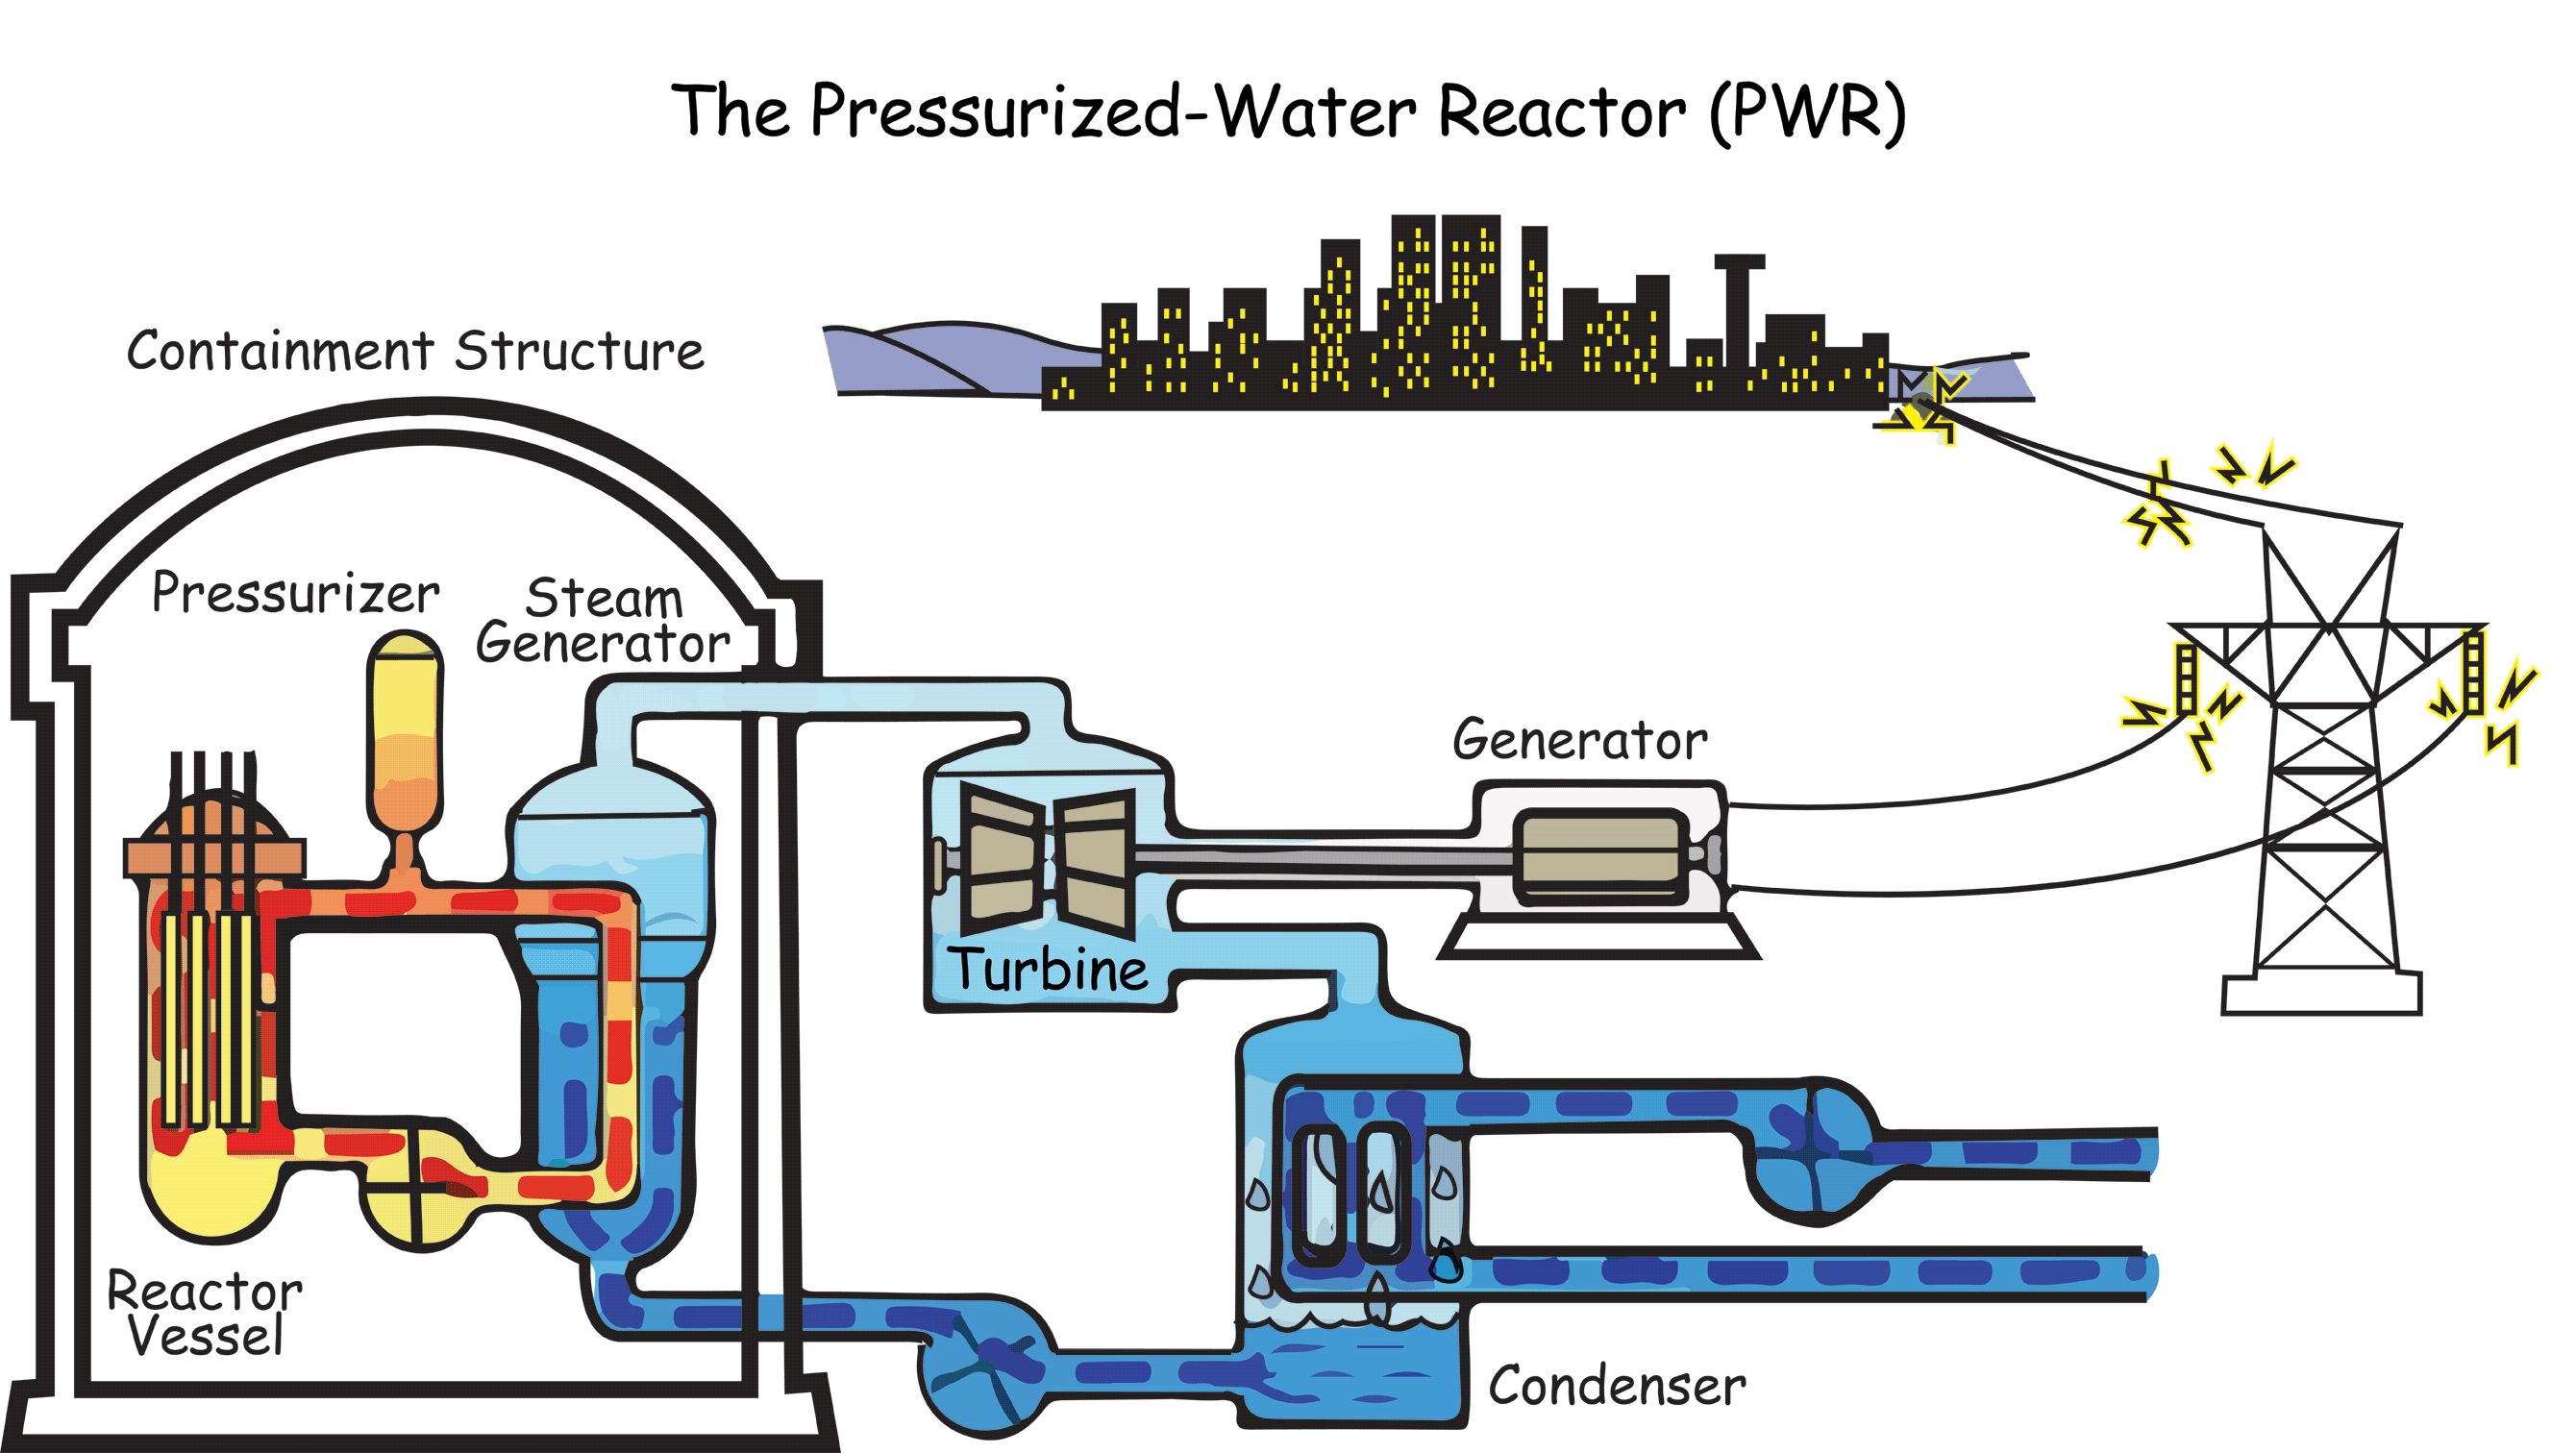
\includegraphics[width=0.75\textwidth]{nukePlan.png}
  \caption{Why are we here?}
\end{figure}
\end{frame}
\begin{frame}[label={sec:orgheadline2}]{Introduction}
\begin{figure}
  \centering
  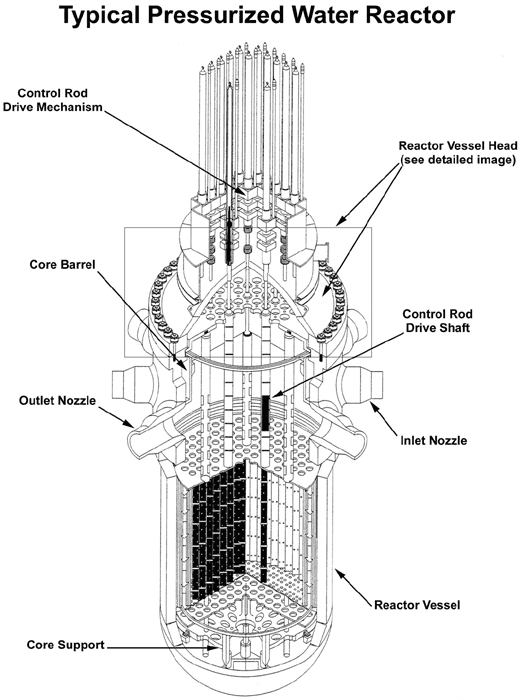
\includegraphics[width=0.45\textwidth]{pwr-rx-vessel-large.png}
\end{figure}
\end{frame}
\begin{frame}[label={sec:orgheadline3}]{Introduction}
\begin{figure}
  \centering
  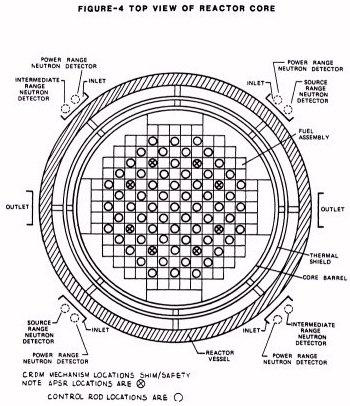
\includegraphics[width=0.55\textwidth]{lwrPlanView.png}
\end{figure}
\end{frame}
\begin{frame}[label={sec:orgheadline4}]{Introduction}
\begin{figure}
  \centering
  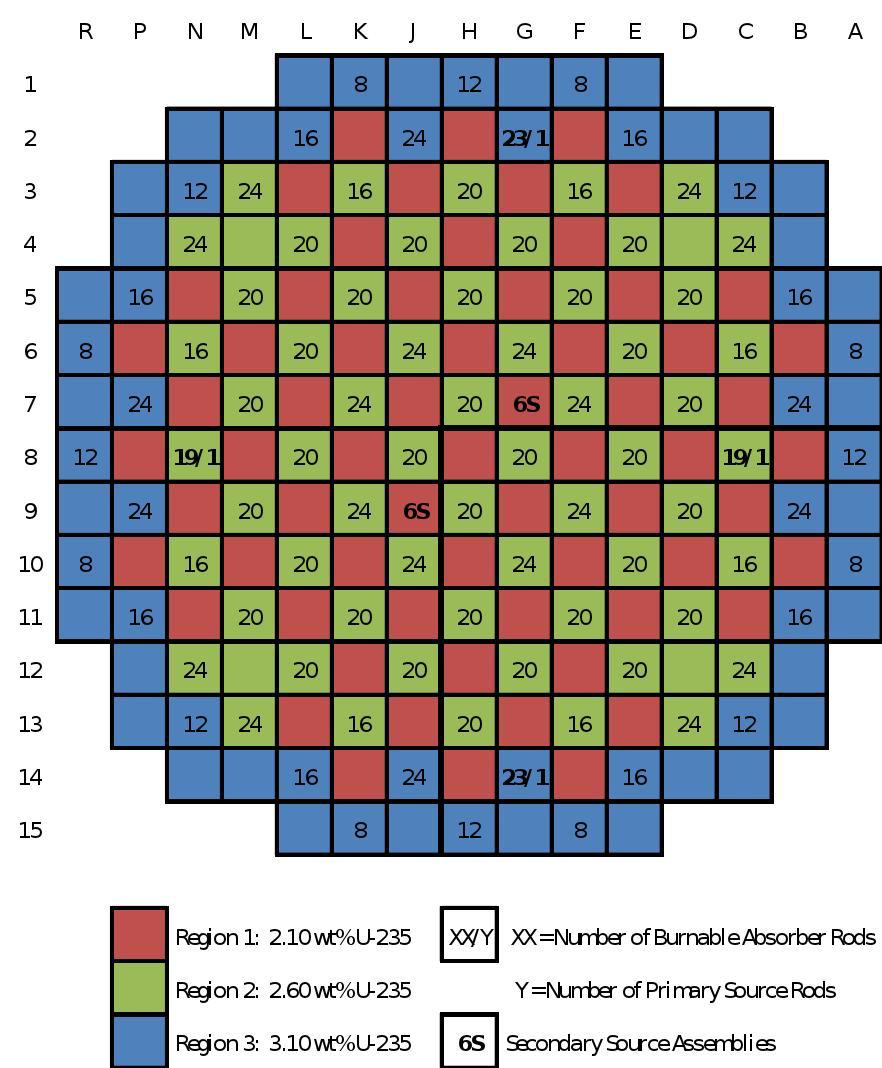
\includegraphics[width=0.55\textwidth]{assemblyGrid.png}
\end{figure}
\end{frame}
\begin{frame}[label={sec:orgheadline5}]{Introduction}
\begin{figure}
  \centering
  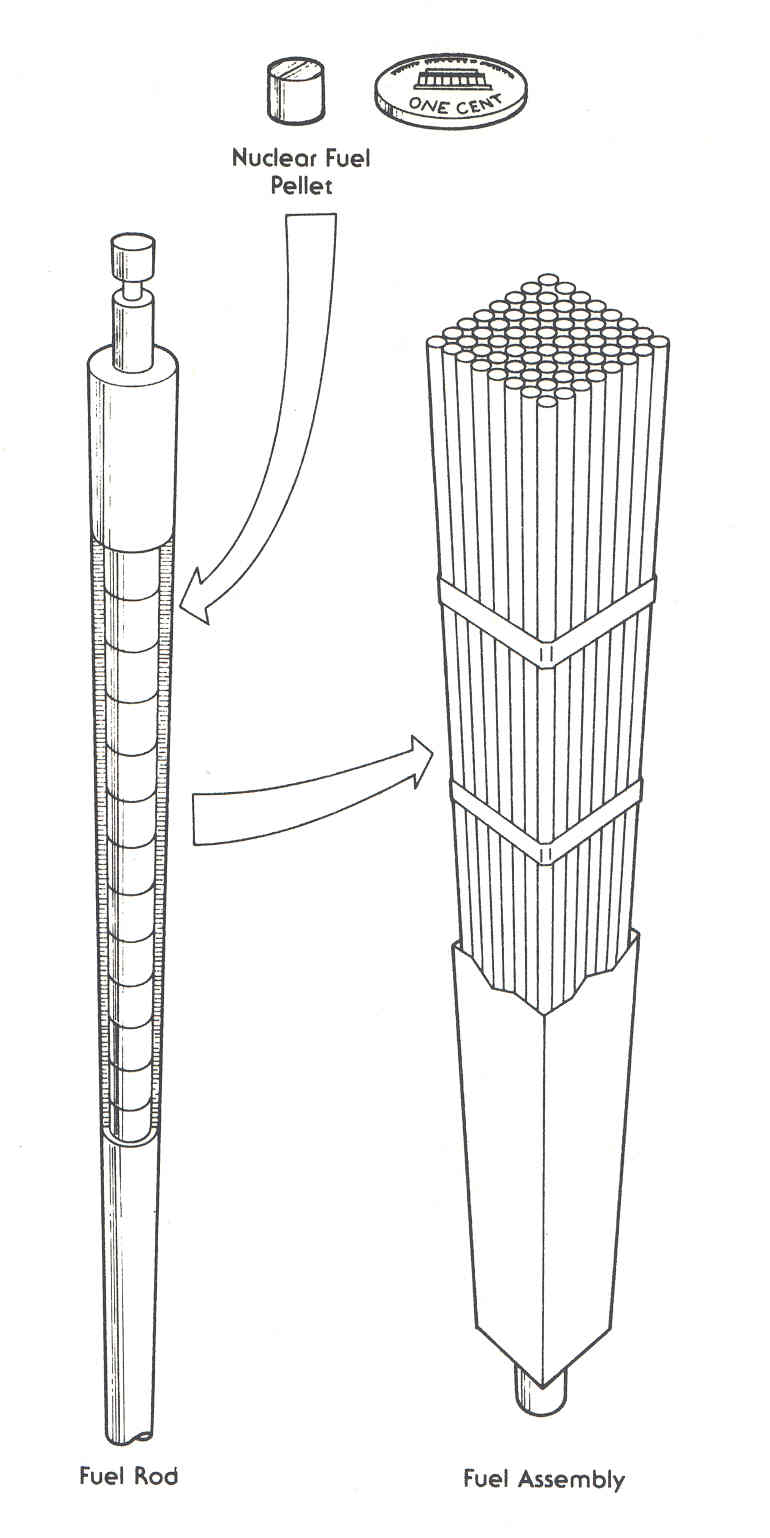
\includegraphics[width=0.35\textwidth]{NEAT22-Figure-1-bwr-fuel-c.png}
\end{figure}
\end{frame}
\begin{frame}[label={sec:orgheadline6}]{Introduction}
\begin{figure}
  \centering
  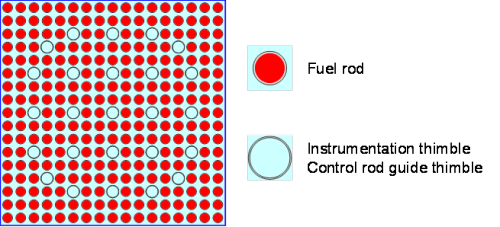
\includegraphics[width=0.75\textwidth]{pwr_fa_17x17.png}
  \caption{PWR assembly geometry.}
\end{figure}
\end{frame}
\begin{frame}[label={sec:orgheadline7}]{Introduction}
\begin{figure}
  \centering
  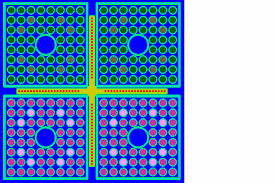
\includegraphics[width=0.75\textwidth]{bwr_fa.png}
  \caption{BWR assembly geometry.}
\end{figure}
\end{frame}
\begin{frame}[label={sec:orgheadline8}]{Introduction}
\begin{table}[]
\centering
\caption{Typical LWR Parameters}
\label{my-label}
\begin{tabular}{|l|c|c|}
\hline
Parameter             & BWR   & PWR   \\
\hline
Rod diameter {[}in{]} & 0.48  & 0.37  \\
Rod height {[}m{]}    & 4.1   & 4.0   \\
Rod pitch             & 0.64  & 0.50  \\
Assembly lattice      & 8x8   & 17x17 \\
\# rods/assembly      & 62    & 264   \\
\# assemblies/core    & 732   & 241   \\
Total \# rods         & 45384 & 63624 \\
\hline
\end{tabular}
\end{table}
\end{frame}
\begin{frame}[label={sec:orgheadline9}]{Energy Self Shielding}
\begin{figure}
  \centering
  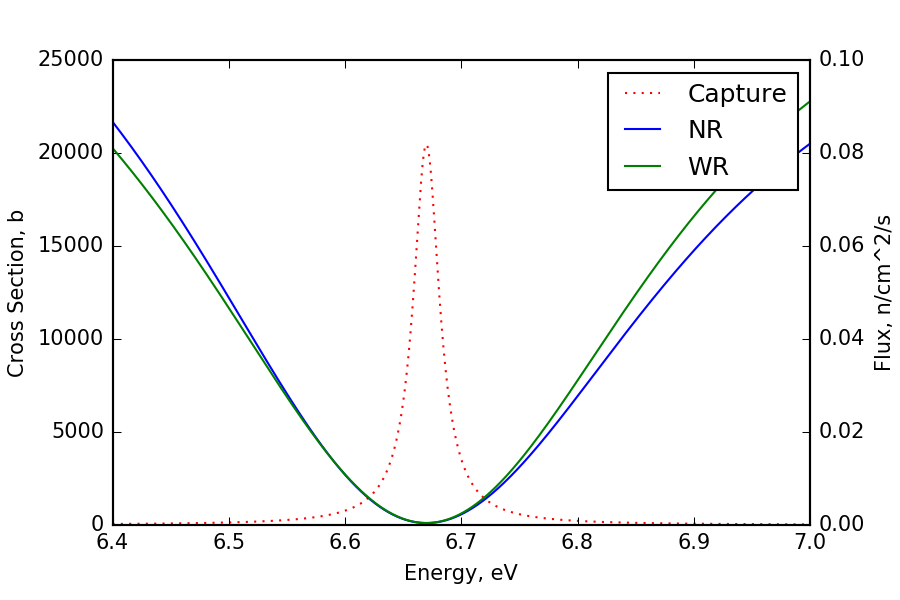
\includegraphics[width=0.75\textwidth]{../notebooks/selfshielding.png}
  \caption{Self shielding of neutron flux in resonance.}
\end{figure}
\end{frame}
\end{document}